%!TEX root = paper.tex

\section{Markov-Chain Monte Carlo}\label{sec:mcmc}

To evaluate the quality of the covariance estimates produced by our method, we used Markov-Chain Monte Carlo (MCMC) as a benchmark for the ``true'' distribution of the logistic regression weights $(w_0, w_1, w_2)$.  We used the \texttt{R} package \texttt{MCMCpack} with an improper uniform prior, 10,000 iterations, and burn-in rate of 1,000 iterations.  We also compared to
an MCMC simulation with a normal prior on the weights $\mathcal{N}(\M{0},1000I)$ and found similar results. Figures~\ref{fig:mcmc_iterations} and \ref{fig:mcmc_iterations_normal} show the progression of the MCMC algorithm assuming each prior.  

\begin{figure}
\centering
	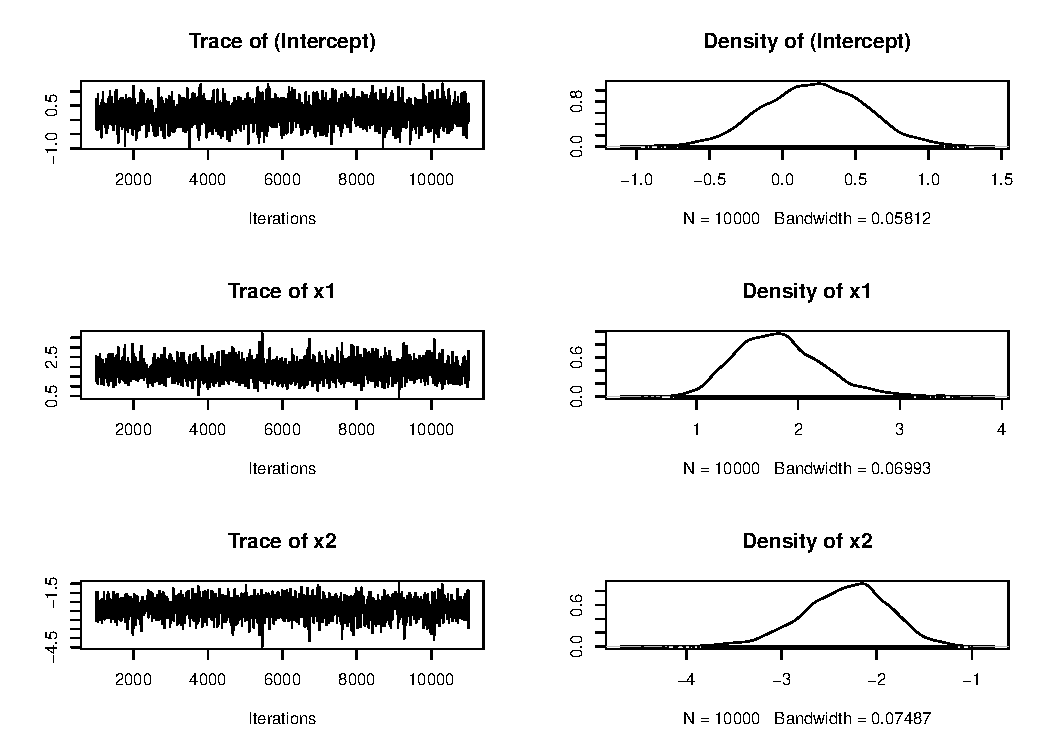
\includegraphics[height=100mm]{figures/mcmc_uniform.pdf}
    \caption{MCMC simulations of logistic regression weights for dataset 1, and corresponding marginal density plots, assuming 
    an improper uniform prior. 10,000 iterations total.}  \label{fig:mcmc_iterations}  
\end{figure}

\begin{figure}
\centering
	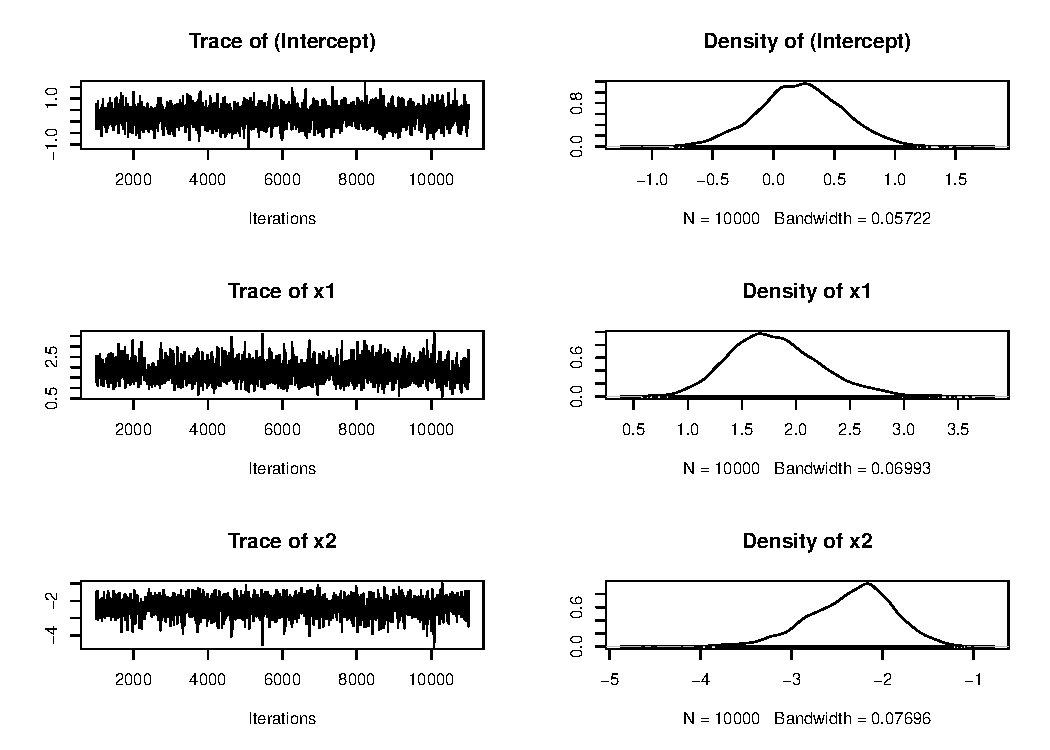
\includegraphics[height=100mm]{figures/mcmc_normal.pdf}
    \caption{MCMC simulations of logistic regression weights for dataset 1, and corresponding marginal density plots, assuming 
    a normal prior $\mathcal{N}(\M{0},1000I)$. 10,000 iterations total.}  \label{fig:mcmc_iterations_normal}  
\end{figure}

To visualize the joint distribution of the logistic regression weights, we plot the MCMC results for the values of $w_1$ and $w_2$.  In addition, we fit the kernel density to the 

<<<<<<< HEAD
%\begin{table}[tb]
\centering
\begin{tabular}{ccc}
  \toprule
  V1 & V2 & V3\\
  \midrule
  0.0566 & -0.0014 & -0.0033 \\
  -0.0014 & 0.0418 & -0.0233 \\
  -0.0033 & -0.0233 & 0.0369 \\
  \bottomrule
\end{tabular}
\caption{caption3}\label{tab:label}
\end{table}

=======
\begin{table}[tb]
\centering
\begin{tabular}{rcccccc}
  \toprule
 {\bf  Dataset} & {\bf  Logit Train} & {\bf  Logit Test} & {\bf  MCMC Train} & {\bf  MCMC Test} & {\bf  MFVB Train} & {\bf  MFVB Test}\\
  \midrule
  0 & 0.8700 & {\bf 0.8580} & 0.8700 & {\bf 0.8580} & 0.8600 & 0.8570 \\
  1 & 0.7500 & 0.8450 & 0.7500 & {\bf 0.8460} & 0.7400 & 0.8450 \\
  2 & 0.5500 & {\bf 0.4890} & 0.5100 & {\bf 0.4890} & 0.5400 & 0.4750 \\
  3 & 0.6900 & {\bf 0.7420} & 0.6900 & {\bf 0.7420} & 0.7200 & 0.7120 \\
  4 & 0.8600 & {\bf 0.8050} & 0.8600 & {\bf 0.8050} & 0.8600 & 0.8040 \\
  5 & 0.9400 & 0.9290 & 0.9400 & {\bf 0.9300} & 0.9400 & 0.9260 \\
  6 & 0.7400 & 0.7130 & 0.7400 & {\bf 0.7140} & 0.6900 & 0.6840 \\
  7 & 1.0000 & 0.9760 & 1.0000 & *** & 1.0000 & {\bf 0.9780} \\
  8 & 0.9200 & {\bf 0.8670} & 0.9200 & {\bf 0.8670} & 0.9300 & 0.8640 \\
  9 & 0.5200 & 0.3980 & 0.5100 & 0.4020 & 0.4600 & {\bf 0.4130} \\
  10 & 0.6700 & 0.6690 & 0.6700 & {\bf 0.6700} & 0.6300 & 0.6560 \\
  \bottomrule
\end{tabular}
\caption{Training and test set accuracy for logistic regression, MCMC logistic regression, and MFVB logistic regression on all datasets.  The highest out-of-sample accuracy score is highlighted for each dataset.  \\ *** : The training dataset was completely separable; therefore the posterior covariance matrix was zero and the precision matrix was undefined.  Thus, we did not obtain MCMC predictive probabilities for this dataset. }\label{tab:all_acc}
\end{table}

>>>>>>> 0a7d1b90b07e73dada71bd4fa5ca4b403dc4fdf1

\begin{figure}
\centering
	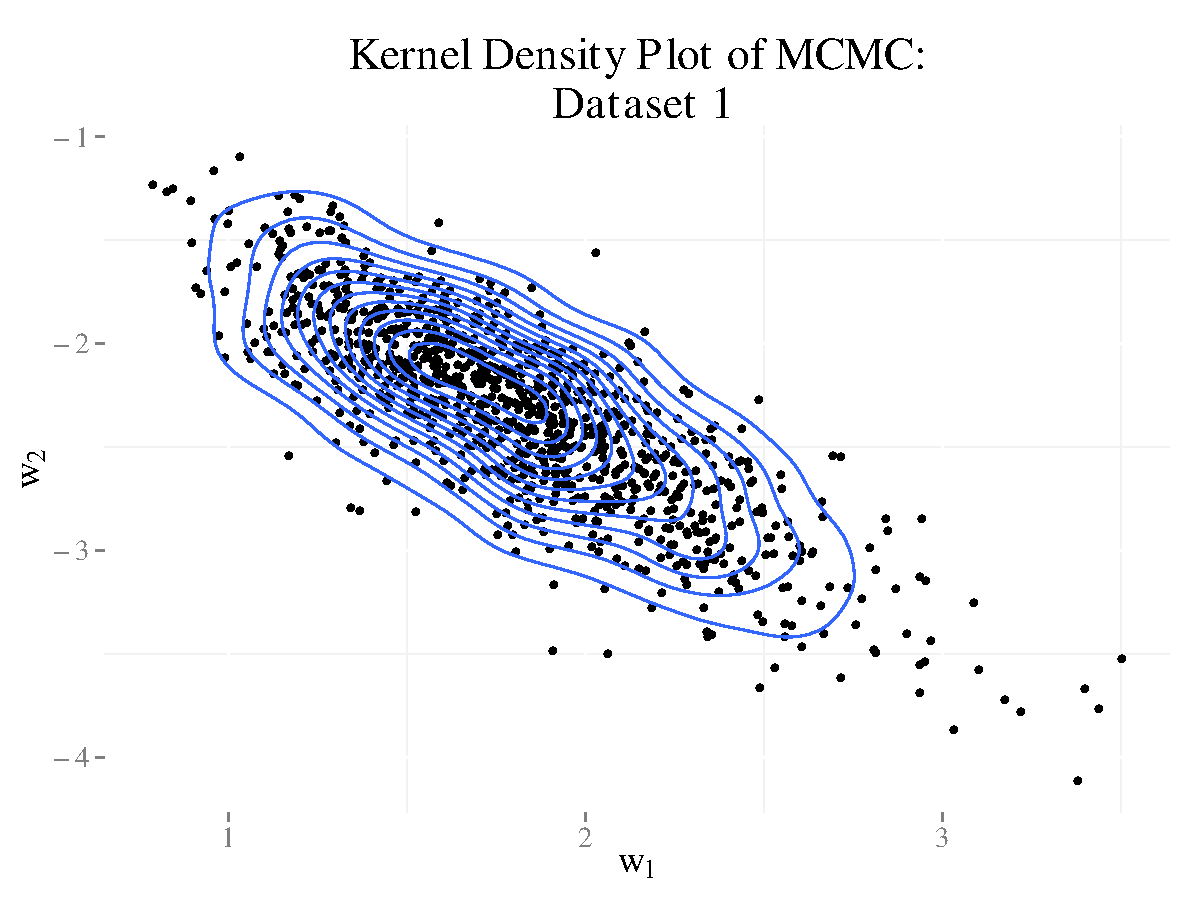
\includegraphics[height=120mm]{figures/mcmc_uniform_2d.pdf}
    \caption{MCMC simulations of logistic regression weights for dataset 1, and corresponding kernel density plot, assuming 
    an improper uniform prior.  Subset of 1,000 out of 10,000 total iterations shown.}  \label{fig:mcmc_kernel}  
\end{figure}

\begin{figure}
\centering
	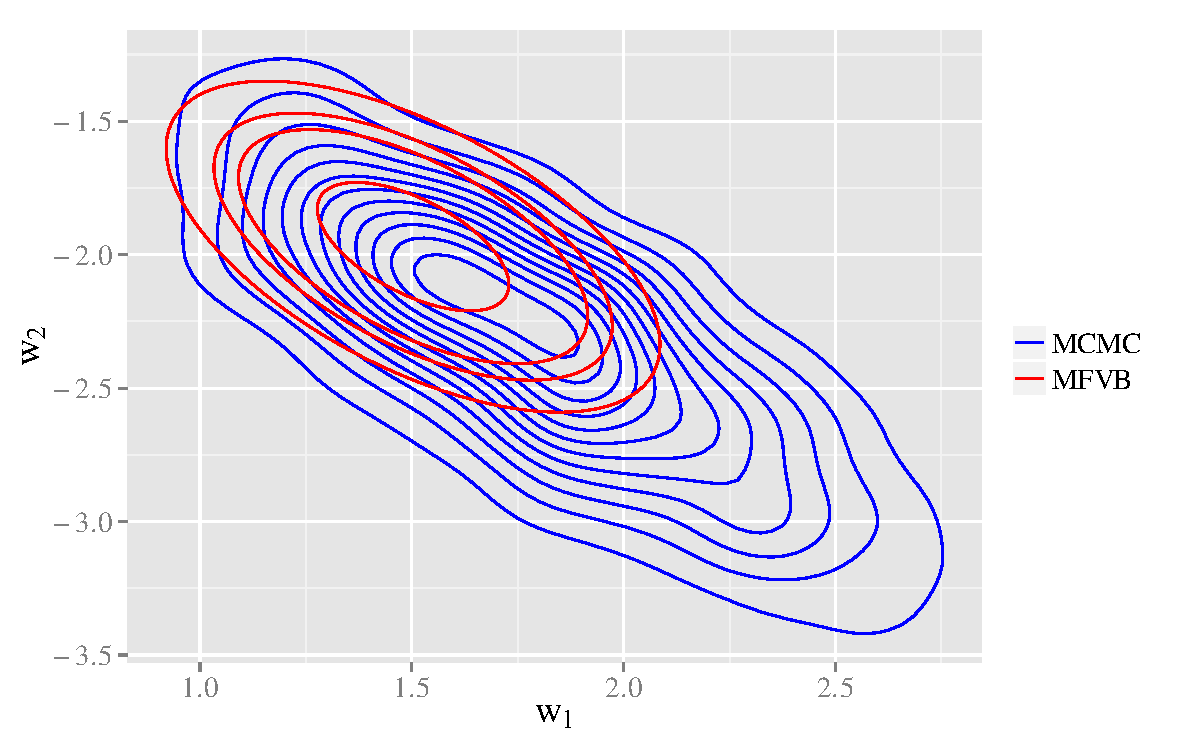
\includegraphics[height=120mm]{figures/mcmc_uniform_mfvb.pdf}
    \caption{Comparison of logistic regression point estimate, kernel density plot of MCMC simulations, and posterior density of
    MFVB logistic regression (vectorized function), for dataset 1.   Contours of MFVB logistic regression indicate
    50\%, 90\%, 95\%, and 99\% confidence intervals for the bivariate normal $\mathcal{N}(\M{w}_{N},\M{V}_N)$.
    Mean values for MCMC and MFVB are also included.}  \label{fig:mcmc_mfvb}  
\end{figure}